\section{Specifying a Tree Datatype}\label{sec:tree}

Tree data structures are useful in many applications: for example, file systems (consisting of directories and files) and XML or JSON documents are trees.
In this section we build upon the data structures of Section~\ref{sec:datatypes} to specify a collaboratively editable tree datatype.
Branch nodes in this tree may be either maps or lists, and leaf nodes are primitive values (wrapped in a $\mathsf{MakeVal}$ operation).

Unlike previous CRDTs for tree data structures \cite{Martin:2010ih,Kleppmann:2016ve}, our datatype supports an \emph{atomic move} operation, which can move an entire subtree to a new location, or rename a key in a map, or reorder items in a list.
Moving an item is not the same as deleting it and re-inserting it in a new location: if two users concurrently delete and re-insert the same item, it would be duplicated.
On the other hand, if two users concurrently move the same item to different locations, the move operation with the greater ID will determine the item's final location.

A tree is a restricted form of the object graph specified in Section~\ref{sec:datatypes}.
First, we require that there is a designated root object: assume that we have an operation ID $\mathsf{root}$ that is less than all other operation IDs (according to the total order on identifiers, introduced in Section~\ref{sec:system-model}).
Further assume that for any OpSet $O$ specifying a tree, we have either $(\mathsf{root},\, \mathsf{MakeList}) \in O$ or $(\mathsf{root},\, \mathsf{MakeMap}) \in O$, depending on whether the root node is a list or a map.
We can then define an object $x$ to be the \emph{parent} of an object $y$ if one of the values in $x$ is a reference to $y$.
The \emph{ancestor} relation is the transitive closure of the parent relation, which we can define using the element relation $E$:
\begin{align*}
    \mathrm{parent}(E,\, i) &=
    \begin{cases}
        \big\{ (\mathit{obj}, \mathit{val}) \mid \exists\,\mathit{id}, \mathit{key}.\;
            (\mathit{id}, \mathit{obj}, \mathit{key}, \mathit{val}) \in E \big\} & \text{if } i=1 \\
        \big\{ (x, z) \mid (x, y) \in \mathrm{parent}(E,\, i-1) \;\wedge\;
            (y, z) \in \mathrm{parent}(E,\, 1) \big\} & \text{if } i > 1
    \end{cases} \\[8pt]
    \mathrm{ancestor}(E) &= \bigcup_{i \;\geq\; 1} \mathrm{parent}(E,\, i)
\end{align*}

An object graph is a tree if the root has no parent, every non-root node has exactly one parent, and if the ancestor relation has no cycles.
We can redefine the operation interpretations from Section~\ref{sec:datatypes-interp} to preserve this tree invariant.
In fact, it is sufficient to redefine the interpretation of $\mathsf{Assign}$, and leave the interpretation of the other five operation types unchanged:
\[
    \mathrm{interp}\big[(E,\, L),\, (\mathit{id},\, \mathsf{Assign}(\mathit{obj}, \mathit{key}, \mathit{val}, \mathit{prev})) \big] \;=\; \left\{
    \arraycolsep=0pt \def\arraystretch{1.5}
    \begin{array}{llllll}
        \multicolumn{2}{l}{(E,\, L)}
        & \text{if } (\mathit{val},\, \mathit{obj}) \in \mathrm{ancestor}(E) \\[8pt]
        \Big( & \multicolumn{2}{l}{
        \big\{ (\mathit{id}', \mathit{obj}', \mathit{key}', \mathit{val}') \in E \mid
        \mathit{id}' \notin \mathit{prev} \;\wedge\; \mathit{val}' \neq \mathit{val} \big\} \;\cup\;} \\
        & \big\{ (\mathit{id}, \mathit{obj}, \mathit{key}, \mathit{val}) \big\},\; L \Big) \qquad
        & \text{if } (\mathit{val},\, \mathit{obj}) \notin \mathrm{ancestor}(E)
    \end{array} \right.
\]

This definition differs in two ways from that in Section~\ref{sec:datatypes-interp}.
Firstly, the operation has no effect if the value $\mathit{val}$ is already an ancestor of the proposed parent $\mathit{obj}$, since the operation would otherwise introduce a cycle.
Secondly, any existing tuple in $E$ that references the same value $\mathit{val}$ is removed, preserving the invariant that every non-root node must have exactly one parent.

Intuitively, this interpretation of $\mathsf{Assign}$ performs an atomic move whenever $\mathit{val}$ is the ID of an existing object in the tree; in that case, it is moved from its existing position to the key $\mathit{key}$ in the object $\mathit{obj}$.
If $\mathit{val}$ does not currently exist in the tree (e.g.\ because it has just been freshly created), the operation behaves like conventional assignment.

\subsection{Discussion: Subtree Move Conflicts}

In a replicated tree datatype that supports move operations, concurrent moves may conflict in various ways \cite{Najafzadeh:2017vk,AhmedNacer:2012us,Tao:2015gd}.
For example, two different operations may concurrently move the same object to different positions; we resolve this conflict by letting the operation with the greatest identifier ``win''.
Intuitively, we can think of the location of an object in the tree as being determined by a last-writer-wins register, and a move operation overwrites that register.

\begin{figure}
\centering
\begin{tikzpicture}
  \tikzstyle{arrow}=[draw,-{Stealth[length=3.5mm]}]
  \node [rectangle,draw] (start) at (4,4) {
      \begin{tikzpicture}
      \node {$\mathsf{root}$} [level distance=9mm] child {node {$a$}} child {node {$b$}};
      \end{tikzpicture}
  };
  \node [rectangle,draw] (left) at (1,2) {
      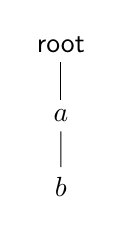
\begin{tikzpicture}
      \node {$\mathsf{root}$} [level distance=9mm] child {node {$a$} child {node {$b$}}};
      \end{tikzpicture}
  };
  \node [rectangle,draw] (right) at (7,2) {
      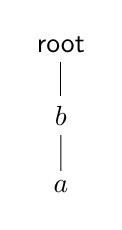
\begin{tikzpicture}
      \node {$\mathsf{root}$} [level distance=9mm] child {node {$b$} child {node {$a$}}};
      \end{tikzpicture}
  };
  \node [rectangle,draw] (merge) at (4,0) { ? };
  \node at (0,4) {$(\mathit{id}_1,\, \mathsf{Assign}(a,\, \mathit{key}_1,\, b,\, \emptyset))$};
  \node at (8,4) {$(\mathit{id}_2,\, \mathsf{Assign}(b,\, \mathit{key}_2,\, a,\, \emptyset))$};
  \draw [arrow] (start.west) -- (left);
  \draw [arrow] (start.east) -- (right);
  \draw [arrow] (left)  -- (merge.north west);
  \draw [arrow] (right) -- (merge.north east);
  \node at (4,1) {merge};
\end{tikzpicture}
\caption{Initially, $a$ and $b$ are siblings. On one node, $b$ is moved to be a child of $a$, while concurrently on another node,
$a$ is moved to be a child of $b$. What should the final outcome be?}\label{fig:concurrent-move}
\end{figure}

A more subtle kind of conflict is illustrated in Figure~\ref{fig:concurrent-move}.
Here, two different objects $a$ and $b$, which are originally siblings, are concurrently moved to be children of each other.
If the move semantics are not defined carefully, it could happen that $a$ and $b$ form a cycle, violating the tree invariant.
Our interpretation function for $\mathsf{Assign}$ handles this situation based on the ordering of the operation IDs $\mathit{id}_1$ and $\mathit{id}_2$.
Since operations are interpreted in order of ascending identifier, one of the two (say, $\mathit{id}_1$) is interpreted first.
When the second ($\mathit{id}_2$) is subsequently interpreted, $a$ is already an ancestor of $b$, and thus the second operation has no effect.

Note that on some nodes, operation $\mathit{id}_2$ may be applied first, and $\mathit{id}_1$ applied later.
In this case, the user will observe first $b$ becoming a child of $a$, and then later observe their positions being swapped (with the effect of $\mathit{id}_2$ being undone).
